\documentclass[12pt]{article}
\usepackage{fullpage}
\usepackage{graphicx, rotating, booktabs} 
\usepackage{times} 
\usepackage{fbb} 
\usepackage{natbib} 
\usepackage{indentfirst} 
\usepackage{setspace}
\usepackage{grffile} 
\usepackage{hyperref}
\usepackage{tikz}
\usepackage[export]{adjustbox}
\usepackage[most]{tcolorbox}
\usepackage{verbatimbox}
\usepackage{lscape}
\usepackage{afterpage}
\usepackage{amsmath}
\usepackage[labelfont={bf},textfont=it,labelsep=period]{caption}
 \usepackage{multirow} 
\setcitestyle{aysep{}}
\usepackage{dcolumn}

\hypersetup{
  colorlinks = true,
  urlcolor = blue,
  linkcolor = black,
  citecolor = black,
  pdfauthor = {Joshua Alley},
  pdfkeywords = {},
  pdftitle = {},
  pdfsubject = {},
  pdfpagemode = UseNone,
%  pdffitwindow = true
%  pdfcenterwindow = true
}



\singlespace
\title{\textbf{Arms Transfers and Electoral Cycles in Trade Between Allies}}
\author{Joshua Alley \\
Postdoctoral Research Associate \\
University of Virginia\thanks{Thanks to Brian Blankenship, Lauren Peritz, Erik Lin-Greenberg, Zachary Markovitch and participants in the Boston University Political Economy of Security Online Workshop Series for helpful comments.} \\
jkalley@virginia.edu
}

 
\date{\today}

\bibliographystyle{apsr}

\usepackage{sectsty}
\sectionfont{\Large}
\subsectionfont{\noindent\large\textit}
\subsubsectionfont{\normalsize}

\makeatletter
\renewcommand\tiny{\@setfontsize\tiny{9}{10}}
\makeatother


\begin{document}

\maketitle 

\begin{abstract}
Military alliances and economic cooperation are inseparable. 
Protege states have strong incentives to engage in the domestic politics of powerful patrons. 
As a result, alliance proteges often use economic ties to advance their security interests by helping patron state leaders create electoral cycles in economic growth. 
U.S. allies do this by purchasing and accepting arms transfers, providing a market for surplus outputs from patron efforts to use defense contracting to stimulate economic growth in key electoral areas.
This paper thus details how alliance proteges use positive economic and security statecraft to help patron state leaders manipulate the economy during leadership competitions.  
I test these claims with three analyses of trade between the United States and its' allies. 
First, I show that U.S. exports to allied states follow an electoral cycle. 
I then detail how arms transfers from the United States to allies mirror electoral export cycles. 
Finally, I show that increased defense contract awards around elections drive greater arms transfers.
These results suggest that alliance patron leaders can reap electoral benefits from security and economic ties with proteges. 
\end{abstract} 


\newpage 
\doublespace 


\section{Introduction}

%% old demands intro
%In 2018, a former Obama administration official argued that ``"Trump is trying to conflate his issues over trade and his beef with Europe and the EU with NATO, and he's using our military strength to do that.''\footnote{\url{https://www.usatoday.com/story/news/politics/2018/07/11/donald-trump-complains-trade-europe-nato-summit/774495002/}}
%In 2019, when Donald Trump claimed that ``It's not right to be taken advantage of on NATO and also then to be taken advantage of on trade, and that's what happens,'' he was neither the first nor the last U.S. policymaker to highlight perceived problematic economic concessions to allies.\footnote{\url{https://www.reuters.com/article/us-nato-summit/very-very-nasty-trump-clashes-with-macron-before-nato-summit-idUSKBN1Y7005}}
%Treasury Secretary John Connally claimed in a 1971 speech that the United States ``had the right to expect more equitable trading arrangements'' with its allies (quoted in \citet[pg 175]{Sayle2019}).
%\footnote{See also: \url{https://www.fpri.org/article/2019/04/the-blue-chip-and-the-little-blue-bird-change-and-continuity-in-nato-policy-from-nixon-to-trump/} and \url{https://history.state.gov/historicaldocuments/frus1969-76v03/d155}}
%More recently, Congressional leaders criticized the Biden administration's decision to waive sanctions on the Nord Stream 2 gas pipeline between Russia and Germany.\footnote{\url{https://www.bbc.com/news/world-us-canada-57180674}}


% start with a good story of increased trade near elections 
% US-Japan 1996? Falls thereafter, only to rise slighly again in 2000 
% coincided with https://www.mofa.go.jp/region/n-america/us/security/security.html 
% https://1997-2001.state.gov/policy_remarks/970415_reis_japan.html (Government procurement was an emphasis) 
% similar pattern in 1980
Exports from the United States to Japan peaked in 1996 at \$108 billion, having risen from \$85 billion in 1992.
This coincided with a crucial joint declaration indicating the the U.S.-Japan alliance would outlast the Cold War. 
It was also the year that Bill Clinton, the architect of the joint declaration and continued U.S. commitment to Japan, stood for reelection. 
U.S. exports to Japan then fell in the subsequent three years, only to rise again by \$7 billion when Vice-President Al Gore ran for President in 2000. 


Increasing U.S. exports to Japan around presidential elections were not a coincidence. 
Japanese policymakers... 


% not sure I want the question:
%This example reflects a general question; when might alliance proteges use economic policy to impact leadership competition in patron states? 
Just as U.S. trade with Japan regularly peaked near U.S. presidential elections, alliance proteges often facilitate electoral trade cycles with their patron.
Electoral export cycles in alliances are the result of arms purchases and transfers. 
Allies take more arms from their patrons near elections because they control this economic tool and patrons use defense contracting to create domestic political business cycles \citep{Tufte1978, Mintz1988, Mayer1995, DerouenHeo2000}. 
Using arms transfers cements cooperative relationships, as it gives patron leaders an economic and political stake in continued alliance participation.


% Findings
I show how allied states facilitate electoral cycles in trade in three ways. 
First, I show that allies receive more U.S. exports as presidential elections approach, contributing to a general electoral trade cycles.
I then show that much of this trade is the result of arms sales and transfers.  
Finally, I show that defense contracting cycles drive U.S. arms exports. 


This argument and evidence build on prior findings that foreign states use economic policies to manipulate electoral competition. 
\citet{KimMargalit2021} find that China reduced Republican vote share in the 2018 midterm elections by targeting trade war tariffs on industries in competitive districts.
In the same way, \cite{ChyzhUrbatsch2021} find that Chinese tariffs on soy reduced Republican vote share in soy-producing areas. 
My argument examines the international security and economic consequences of domestic political budget cycle policies.


% economic and seucrity ties 
The argument and findings address three salient issues in international relations theory and practice. 
First, they speak to debates about how economic and security ties interact \citep{Mastanduno2009, Poast2019}. 
Scholars dispute whether economic linkages drive security ties \citep{BiglaiserDeRouen2007, Fordham2010, Kimball2010}, security concerns encourage economic linkages \citep{Gowa1995, Li2003, LongLeeds2006, GowaMansfield2004}, or both \citep{BiglaiserDeRouen2009, KinneBunte2018}. 
My findings suggest that in some alliances, this relationship changes with leadership competition as allies adjust their policies to electoral cycles.


Research on economic bargaining in asymmetric alliances usually focuses on patron states' economic leverage, and falls into two camps. 
One argues that alliance patrons have limited economic leverage because they prioritize geopolitical aims \citep{Drezner2013, WolfordKim2017}.
Another perspective claims that alliance leaders have substantial economic influence \citep{Norrlof2010, Brooksetal2013} and threats to reduce security commitment encourage economic concessions \citep[pg. 122]{Oatley2015}.
Rather than focus on economic demands by the patron, my argument suggests that proteges receive arms transfers to help patron leaders advance their electoral interests.


% economic cycles
Expanded exports from alliance patrons to proteges in election years also bolster political business cycles where elites manipulate economic policy to win reelection. 
Elected leaders often use fiscal \citep{Rogoff1987} and monetary policy \citep{ClarkHallerberg2000} to generate economic growth around elections. 
Defense spending, especially contracting, is an especially flexible fiscal tool \citep{Tufte1978, Mintz1988, Mayer1995, DerouenHeo2000, Becker2021}.
There is also evidence that leaders use non-budget instruments like social policy \citep{Philips2020}, labor agreements \citep{Ahlquist2010} and trade disputes \citep{Conconietal2017} to win elections. 


In addition to standard domestic mechanisms, other countries can facilitate political budget cycles. 
International economic expansions and related domestic growth make early elections in parliamentary democracies more likely \citep{Kayser2006} and vote shares for parties supporting higher taxes and spending \citep{Kayser2009}.
For large countries like the United States, domestic political business cycles reshape international economic ties.


% coercion
Finally, this paper provides new insight into economic statecraft. 
Most economic statecraft scholarship examines economic sanctions (e.g. \citep{Marinov2005, Allen2008, Escriba-FolchWright2010}).
But as \citep{Baldwin2020} notes, economic statecraft includes positive inducements and negative sanctions. 
This paper examines positive economic statecraft--- how alliance proteges use political economy decisions to reward patron leaders.
As a result, it assesses issue linkage in alliance management, building on previous work that considers alliance formation \citep{Poast2012} and credibility \citep{Davis2008, Poast2013}. 


% policy 
My findings that allies facilitate political budget cycles through arms exports has important implications for alliance durability. 
Leaders who anticipate benefiting from allied trade cycles will be more likely to demonstrate and uphold alliance commitment. 
Electoral trade cycles are therefore an important component of potential grand bargains between asymmetric alliance patrons and their proteges. 


% need an outline 
The paper proceeds as follows. 
To start, I outline an argument detailing the potential international consequences of political business cycles in large alliance patrons and how allies can use arms imports to support patron leaders. 
I then test detail the process with three pieces of evidence. 
First, I show that U.S. exports to allies increase more as elections approach, relative to states without a defense pact. 
I then demonstrate that arms exports from the United States to allies mirror the electoral export cycle almost exactly.
Finally, I establish the political business cycle roots of arms exports with an analysis of defense contracting and arms exports.
The last section discusses the results and offers some concluding thoughts.


\section{Argument}


This argument explains how alliance proteges facilitate patron political business cycles through arms transfers. 
First, I detail prior findings about political budget cycles and how direct leader control makes defense contracting an attractive policy tool for these cycles. 
Then, I explain how allies provide an market for outputs from electoral cycles in defense contracting. 
Finally, I detail the final outcome--- electoral cycles in trade with allies. 


% basic asymm alliance framework
In asymmetric alliances between large and small states, the large state protects its junior partner in exchange for foreign policy concessions \citep{Morrow1991}.
A credible promise of military support increases the large state's foreign policy influence. 
Small alliance members garner protection from external threats and sacrifice some foreign policy autonomy. 
Although many asymmetric alliance formalize hierarchical relationships, security and economic hierarchy are distinct \citep{Lake2009}. 


Military alliances and economic cooperation are inseparable.
Many alliances also include explicit or implicit promises of economic cooperation \citep{GowaMansfield2004, LongLeeds2006, Davis2008, Poast2012}.\footnote{Conflict and economic integration are linked in general (see for example, \citep{GartzkeLi2003, Chen2021}).}
Prior research indicates that alliances promote trade \citep{Gowa1995, GowaMansfield2004, Haim2016} or protect existing trade ties \citep{Fordham2010}.
Alliances also encourage foreign direct investment \citep{LiVashchilko2010} and monetary cooperation \citep{Li2003}.
A cooperative bargain of security and economic ties results. 


% Political Business cyles
Close economic ties make alliance proteges more sensitive to economic conditions in their patron.
Fiscal and monetary policy shifts in the patron impact economic activity, which then transmits into proteges through trade and financial ties. 
Economic interdependence leads to correlated economic growth across countries \citep{ArtisZhang1999, Kayser2006} and increases the global influence of large economies like those of most alliance patrons.


Economic policy in democratic alliance patrons changes with electoral cycles.
In anticipation of elections, leaders undertake political business cycles by using fiscal and monetary policy to increase economic growth \citep{Tufte1978, Rogoff1987}. 
Given strong central bank interdependence, which is common in most alliance patrons, fiscal cycles are more likely \citep{ClarkHallerberg2000}. 


% targeted and flexible policies 
Fiscal and monetary policies are relatively blunt policy instruments, however. 
Aggregate budgets have less flexibility, as leaders often lack discretion in how to spend allocated resources. 
As a result, leaders use other policies such as trade disputes \citep{Conconietal2017}, labor agreements \citep{Ahlquist2010} and land reform \cite{Philips2020} to win support in key constituencies. 


% Defense spending/contracts as flexible instrument
Within fiscal policy, defense spending is more flexible than some other areas of the budget.
Executive leaders often have more discretion in how to allocate defense resources.
\citet{WhittenWilliams2011} note that defense spending can serve social welfare goals. 
\citet{Becker2021} finds that unemployment in NATO members encourages leaders to shift spending from equipment to personnel.
Electoral cycles in defense spending follow \citep{Tufte1978, Mintz1988}.


% in US context, contracts
More recent work on the United States argues that defense budgets, which are set two years in advance, are not pliable enough to drive political cycles.
As a result, attention shifted towards defense contracting, as leaders have more control over contract timing and disbursement \citep{Mayer1995, DerouenHeo2000}.
Disbursing contracts allows leaders to target key constituencies in response to unemployment and approval shifts.


% increased production of arms- not tied to security needs
Defense contracting increases arms production by employing firms to produce defense goods. 
While these goods can equip the patron state military, electoral cycles and defense planning may diverge.
Put differently increased supply from electoral cycles in defense contracting does not respond to increased demand from the patron state military. 
As a result, foreign markets provide fresh demand and outlets for additional arms production under defense contracting cycles. 


% potential markets: allies
% take new or used stuff to make room
Allies are the obvious market for outputs from political cycles in defense contracting.
Close security cooperation and economic integration of defense industries create economic and security ties that encourage arms trade \citep{Bitzinger1994}. 
\citet{Thurneretal2019} find that the relative importance of security and economic factors fluctuates, but alliances consistently increase arms transfers.


% positive statecraft tie-in from Baldwin 


% Sales and transfers- who pays for what


% sending arms: political benefits for patron and proteges
Electoral cycles in arms transfers thus have political benefits for patron and protege leaders.
Patrons gain additional flexibility to manipulate economic conditions.
Proteges curry favor with their patron, bolster their military capabilities and deepen perceived commitment. 
\citet{McManusYarhi-Milo2017} argue that arms transfers are a costly but less visible signal of patron support.\footnote{\citet{Yarhi-Miloetal2016} argue that arms transfers sometimes substitute for alliances so patrons can provide security with less entrapment risk.}


% less export cycles to non-allies
The security externalities of arms transfers will reduce electoral cycles in arms exports to non-allies. 
Patron states will be less willing to increase the capability of potential opponents, even if it facilitates electoral cycles.
Limited defense industry cooperation also constrains the set of potential exports to finished goods, while allies with defense industrial ties can send intermediate goods.


Arms transfers also fall under direct leader control in the protege, which gives leaders flexibility to respond to defense contracting cycles in their patron.
Arms imports are more flexible than trade policy. 
To give a related example, political control over firms increases trade policy flexibility \citep{Davisetal2019}.
As the customer for arms, the protege government has direct control over import decisions.


% increased domestic consumption- imports rise
Electoral cycles in fiscal and monetary policy impact other trade ties as well. 
Greater economic growth from political budget cycles increases domestic consumption.
This increases demand for imported goods. 
Electoral cycles in imports follow, as consumption shifts with economic expansions and contractions from political budget cycles.  


% Net implications: total trade increases and trade balances unchanged


% Result- increased exports, tied to electoral cycles
The result of this process is increased exports from alliance patrons to their proteges as elections approach.
These electoral export cycles in alliances are the result of arms transfers. 
Arms transfers in turn are rooted in electoral cycles of defense contracting.





\subsection{Implications}



The argument generates several testable implications. 
Testing is most straightforward in states with a fixed electoral calendar and robust domestic defense industry. 
Therefore, this analysis focuses on the United States, which also has clear evidence of defense contracting cycles.


The first hypothesis predicts electoral cycles in trade generally. 
As presidential elections approach, I expect increasing exports from the United States to alliance proteges.
Because arms exports drive this cycle, I expect that it holds primarily in allies.


\begin{quote}
\textsc{Export Cycles Hypothesis: As time to a presidential election decreases, U.S. exports to junior allies will increase.}
\end{quote}



The second hypothesis predicts corresponding cycles in arms transfers.
If arms transfers and sales drive export cycles, electoral cycles in arms transfers should match trade cycles.
Proximity to presidential elections will increase arms transfers from the United States to allied states. 


\begin{quote}
\textsc{Arms Transfers Hypothesis: As time to a presidential election decreases, U.S. arms transfers to junior allies will increase.}
\end{quote}


The third prediction tests the expected relationship between defense contracts and arms exports. 
I expect electoral cycles in defense contacting, and a positive correlation between these cycles and U.S. arms transfers.


\begin{quote}
\textsc{Defense Contracts Hypothesis: As defense contracting increases around elections, U.S. arms transfers will increase.}
\end{quote}



In the following, I describe how I test each of these hypotheses. 
In the first analysis, I establish the role of allies in electoral export cycles. 
The second analysis shows increasing exports to allies track with the U.S. electoral cycles, and are of comparable magnitude to trade cycles.
Finally, I test the final link in the argument chain with an analysis of defense contracting and arms exports from YEAR TO YEAR.




\section{Electoral Cycles in U.S. Exports to Allies}

To test the first hypothesis, I analyze U.S. trade from 1950 to 2014. 
This analysis presents electoral trade cycles, then establishes that allies drive electoral export cycles.
The key independent variable is a dummy indicator of a defensive alliance between the United States and each state, drawn from the ATOP database \citep{Leedsetal2002}.
I then employ elections data from the National Elections across Democracy and Autocracy (NELDA) dataset \citep{HydeMarinov2012} to identify presidential election years and calculate years to the election.
The years to election variable ranges from zero in election years to three in the year immediately after an election.
Finally, I interact the defensive alliance dummy with the years to election variable.


For U.S. exports, my argument makes three predictions about the interaction between alliances and years to election. 
First a positive constituent term on the defensive alliance variable, which indicates that allies take more exports than non-allies in election years, when time to election is zero.
Second, I expect a negative constituent term on years to election as non-allied states respond to political business cycles in other ways.
Last, and most importantly, a negative interaction between alliances and time to the election, which suggests that exports to allies are more responsive to elections than exports to states without a defensive alliances with the United States.


The key outcome is annual changes in the natural log of exports, but I also model changes in total trade, imports, and the trade balance to assess the net impact of export changes.
I use changes because models in levels with a lagged dependent variable suggest non-stationarity in many panels. 
Because lagged trade flows have unit roots or near unit root coefficients, models in levels risk spurious inferences.
I draw on exports and imports data from the IMF's direction of trade statistics database.


In addition to the interaction of time to elections and a defensive alliance, I include a series of control variables that may be correlated with alliances and trade. 
Key trade variables include for changes in the GDP of both states, population-weighted distance, contiguity, common language and former colonial ties \citep{FouquinHugot2016}.
I also adjust for democracy \citep{Marquez2016}, the presence of a militarized interstate dispute \citep{Gibleretal2016}, and shared IGO membership \citep{Pevehouseetal2020}.\footnote{Some dyadic data from the \textit{peacesciencer} \textsf{R} package \citep{peacesciencer-package}.}


Some trade flow changes are unusual. 
This creates heavy-tailed residuals, so I employ a robust regression estimator; M-estimation with Tukey's biweight function \citep{RaineyBaissa2020}.
Robust regression places less weight on unusual observations, making it more efficient than OLS for this particular outcome.



\subsection{Results}


Raw trade data clearly shows electoral cycles in U.S. exports, imports and total trade. 
\autoref{fig:us-trade-cycles} presents the distribution of changes in exports, imports and overall trade in years with differing electoral proximity.
Box plots summarize the distribution of U.S. trade with all states in those years. 
The dark line in each box plot marks the median value. 



\begin{figure}
\centering
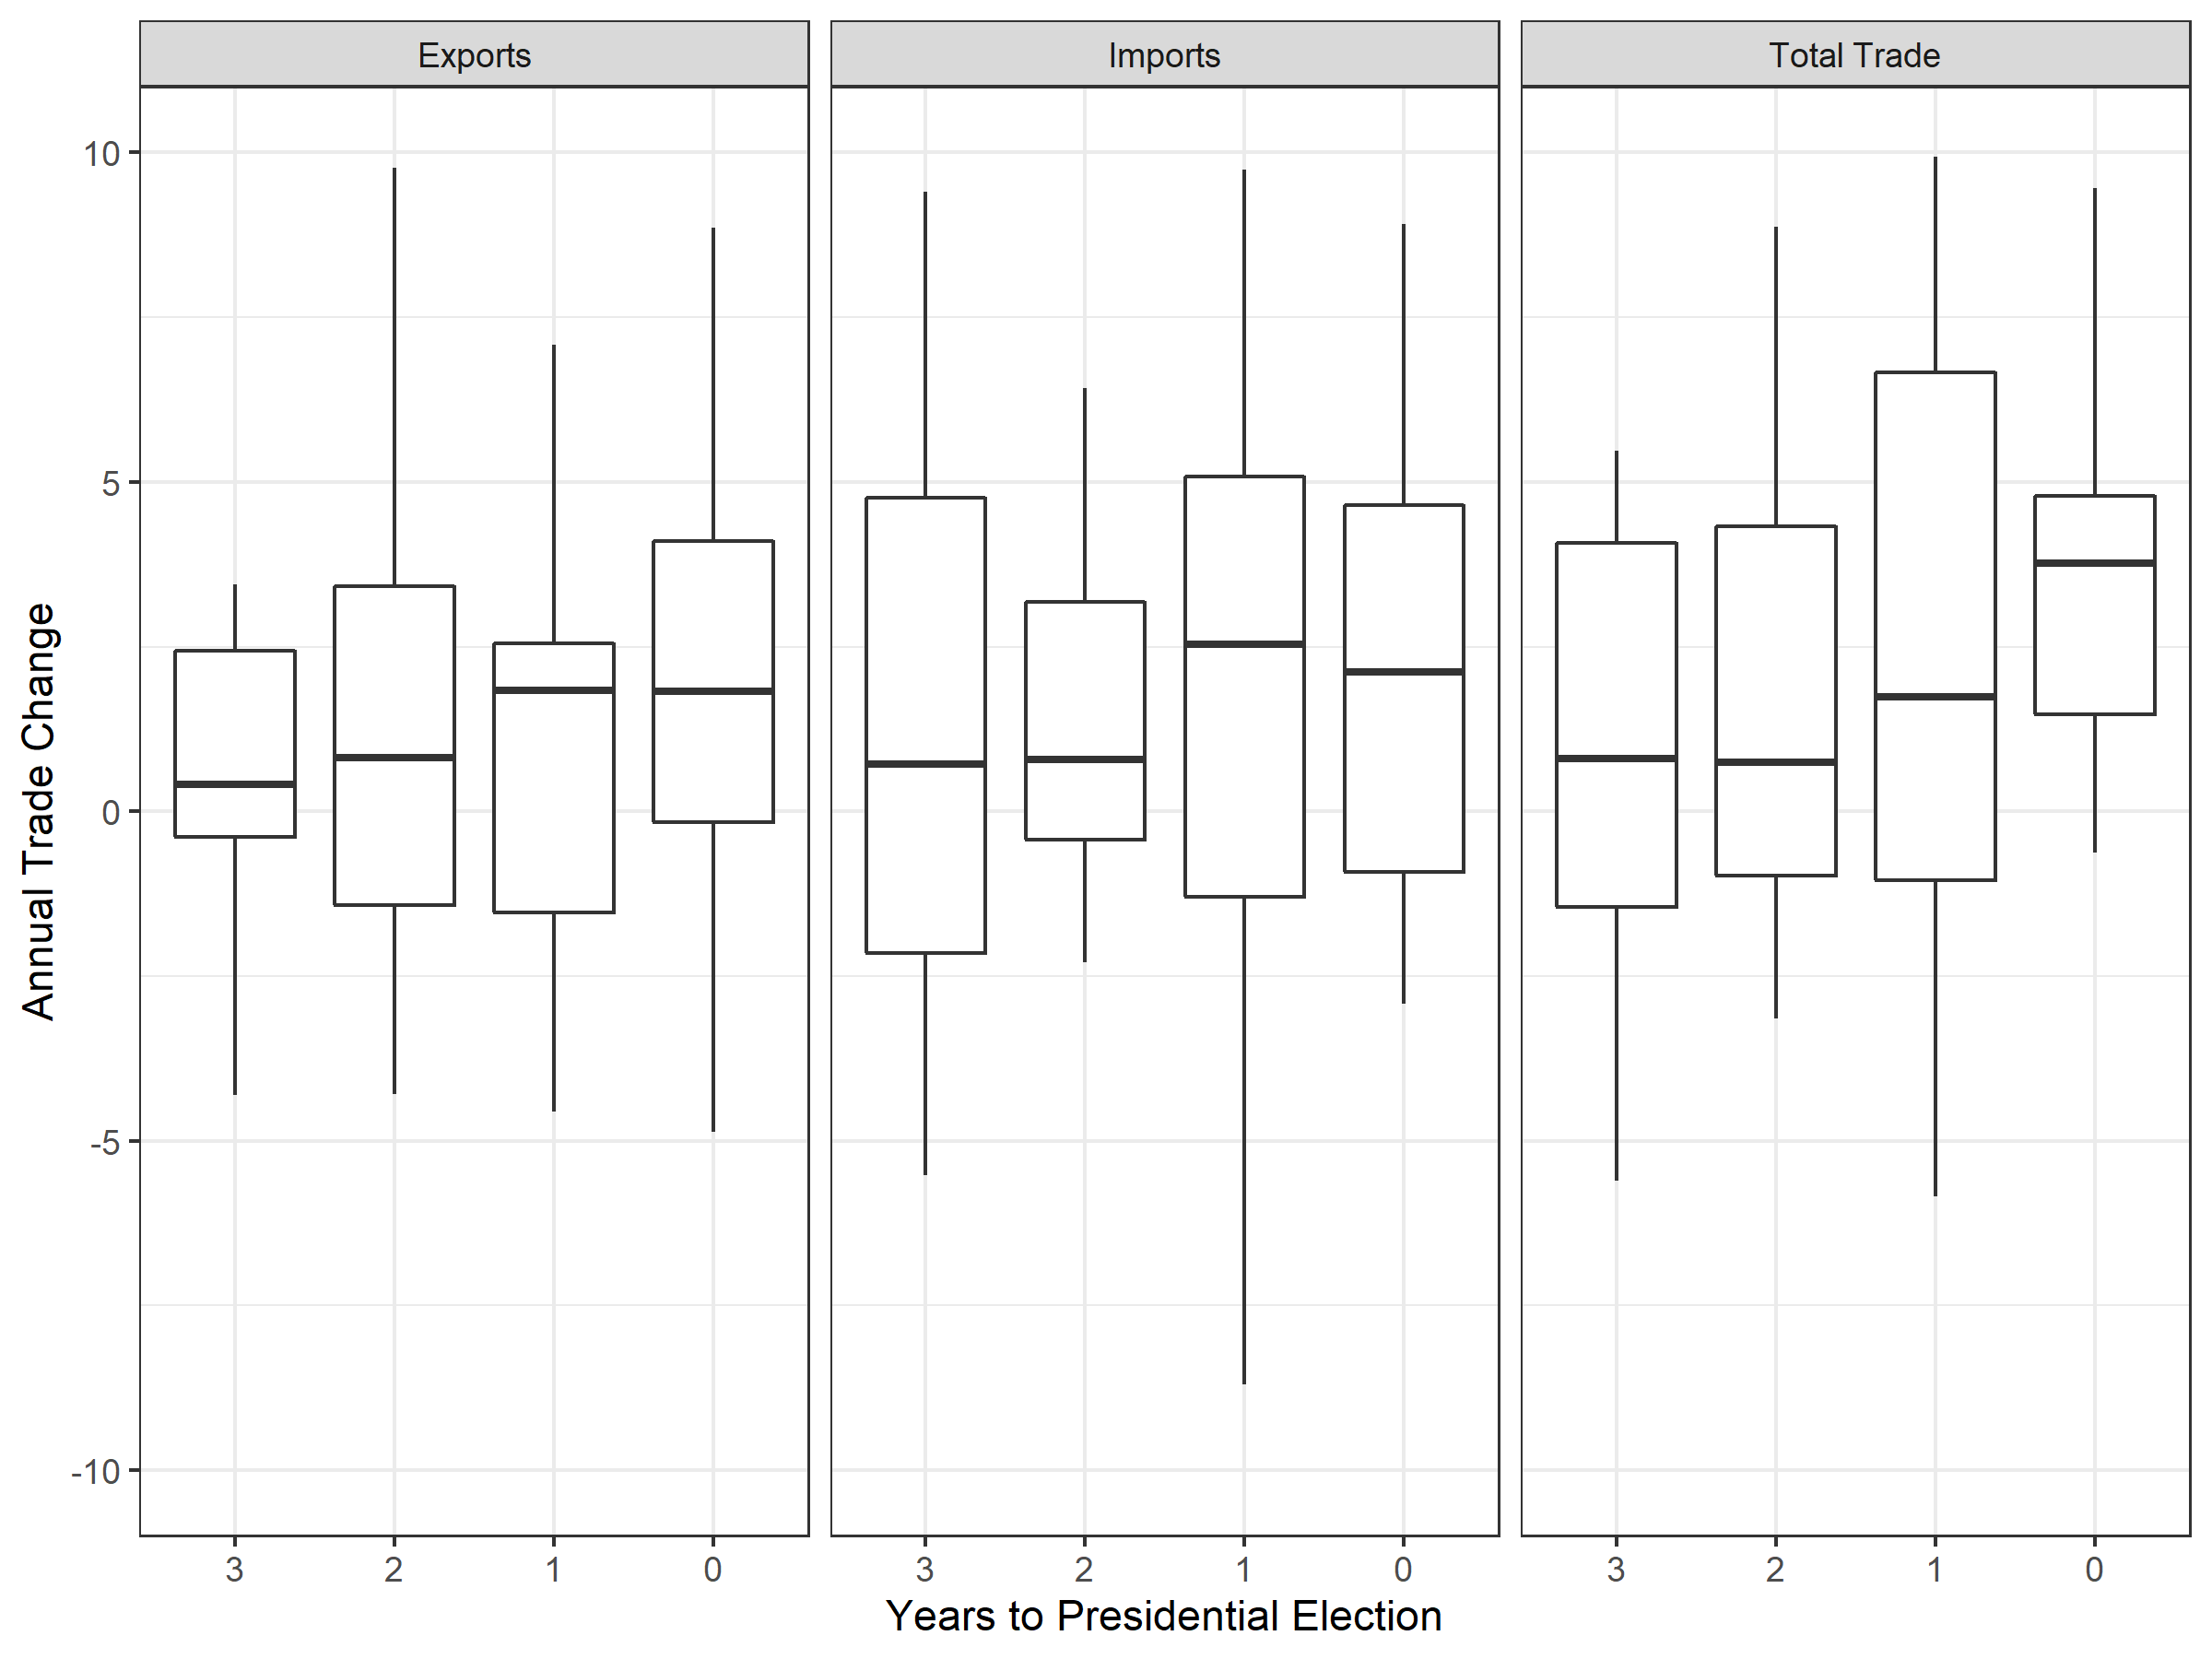
\includegraphics[width=0.95\textwidth]{../figures/us-trade-cycles.png}
\caption{Electoral cycles in U.S. trade between 1950 and 2014. Each box plot summarizes the distribution of changes in logged exports, imports, and overall trade as a presidential election approaches. The thick black line in each plot marks the median value.}
\label{fig:us-trade-cycles}
\end{figure}


While there is ample variation in export changes across all years, the median change in exports is higher in the year before or year of a presidential election.
Imports also rise, though they are extremely variable in the year before an election. 
As a result of increasing exports and imports, total trade often increases, especially in presidential election years.


\autoref{fig:us-trade-cycles} shows electoral cycles in U.S. trade, but it does not clarify which states are driving those trade differences. 
\autoref{tab:us-trade-coefs} presents coefficient estimates from the robust regression models. along with 95\% confidence intervals in parentheses. 
These estimates suggest that allies drive U.S. export cycles, but all states respond to elections with increased exports to the United States. 


\begin{table}
\centering
\resizebox{\textwidth}{!}{ 
\begin{tabular}[t]{lcccc}
\toprule
  & Change Exports & Change Imports & Change Trade & Change Balance\\
\midrule
Defense Pact & 0.013 & 0.008 & 0.013 & 0.012\\
 & (0.005, 0.021) & (0.001, 0.015) & (0.004, 0.022) & (-0.006, 0.031)\\
Defense Pact x Years to Election & -0.006 & 0.000 & -0.003 & -0.007\\
 & (-0.009, -0.002) & (-0.004, 0.003) & (-0.008, 0.001) & (-0.015, 0.002)\\
Years to Election & -0.001 & -0.004 & -0.007 & 0.005\\
 & (-0.003, 0.001) & (-0.006, -0.002) & (-0.009, -0.004) & (0.000, 0.011)\\
Allied Democracy & -0.003 & -0.001 & -0.001 & 0.002\\
 & (-0.008, 0.002) & (-0.006, 0.004) & (-0.007, 0.005) & (-0.011, 0.014)\\
Change Major Power GDP & -0.024 & -0.009 & -0.026 & -0.014\\
 & (-0.028, -0.020) & (-0.013, -0.005) & (-0.031, -0.021) & (-0.024, -0.004)\\
Change Ally GDP & 0.016 & 0.003 & 0.014 & 0.008\\
 & (0.012, 0.020) & (0.000, 0.007) & (0.009, 0.018) & (-0.001, 0.018)\\
Pop. Weighted Distance) & 0.000 & 0.007 & 0.004 & -0.009\\
 & (-0.005, 0.005) & (0.003, 0.012) & (-0.001, 0.010) & (-0.021, 0.002)\\
Contiguous & 0.017 & 0.026 & 0.023 & -0.020\\
 & (0.001, 0.033) & (0.011, 0.040) & (0.005, 0.041) & (-0.058, 0.017)\\
Common Language & 0.004 & -0.005 & -0.002 & 0.011\\
 & (0.000, 0.008) & (-0.009, -0.001) & (-0.007, 0.003) & (0.001, 0.021)\\
Former Colony & -0.004 & 0.003 & -0.004 & -0.007\\
 & (-0.015, 0.007) & (-0.007, 0.014) & (-0.017, 0.009) & (-0.033, 0.020)\\
Ongoing MID & -0.025 & -0.020 & -0.036 & 0.007\\
 & (-0.039, -0.011) & (-0.033, -0.007) & (-0.052, -0.020) & (-0.026, 0.040)\\
Shared IGOs & 0.009 & 0.017 & 0.011 & -0.023\\
 & (0.002, 0.015) & (0.012, 0.023) & (0.004, 0.018) & (-0.038, -0.008)\\
EU Member & 0.002 & 0.005 & 0.007 & -0.012\\
 & (-0.008, 0.011) & (-0.003, 0.014) & (-0.004, 0.018) & (-0.034, 0.011)\\
Cold War & 0.006 & -0.006 & 0.004 & 0.009\\
 & (0.001, 0.011) & (-0.010, -0.002) & (-0.001, 0.010) & (-0.003, 0.020)\\
Republican President & -0.001 & -0.008 & -0.007 & 0.006\\
 & (-0.005, 0.003) & (-0.012, -0.005) & (-0.011, -0.002) & (-0.003, 0.016)\\
Change Ln(Imports) & 0.159 &  &  & \\
 & (0.145, 0.173) &  &  & \\
Change Ln(Exports &  & 0.146 &  & \\
 &  & (0.132, 0.161) &  & \\
\midrule
Num.Obs. & 7161 & 7161 & 7161 & 7161\\
\bottomrule
\end{tabular}
}
\caption{Robust regression coefficients from models of U.S. trade, 1950 to 2014. 95\% confidence intervals in parentheses.}
\label{tab:us-trade-coefs}
\end{table}



As expected, the interaction between the defensive alliance dummy and years to election is negative, which implies that allies receive more U.S. exports as presidential elections approach.
Allies receive more U.S. exports in general, and respond especially strongly to elections when doing so.


The interaction term for imports suggests no clear difference in U.S. imports around elections between allies and non-allied states. 
Moreover, the time to election constituent term is negative for all outcomes, except the trade balance. 
Trade changes approximate the track of exports. 
Simultaneous increases in imports and exports have a more uncertain impact on trade balances.
 


% predicted
The sign and confidence intervals of the interaction terms are inadequate evidence of a conditional relationship \citep{BramborClarkGolder2006}, so I plot predicted changes in trade flows in \autoref{fig:us-elec-pred}.
This figure presents predicted changes in trade across time to election for states with and without a U.S. defense pact. 
Given non-linear relationships from logged trade flows and a robust estimator, these predictions are more straightforward to interpret than marginal effects.\footnote{I present marginal effects in the appendix.} 


\begin{figure}[htpb]
	\centering
		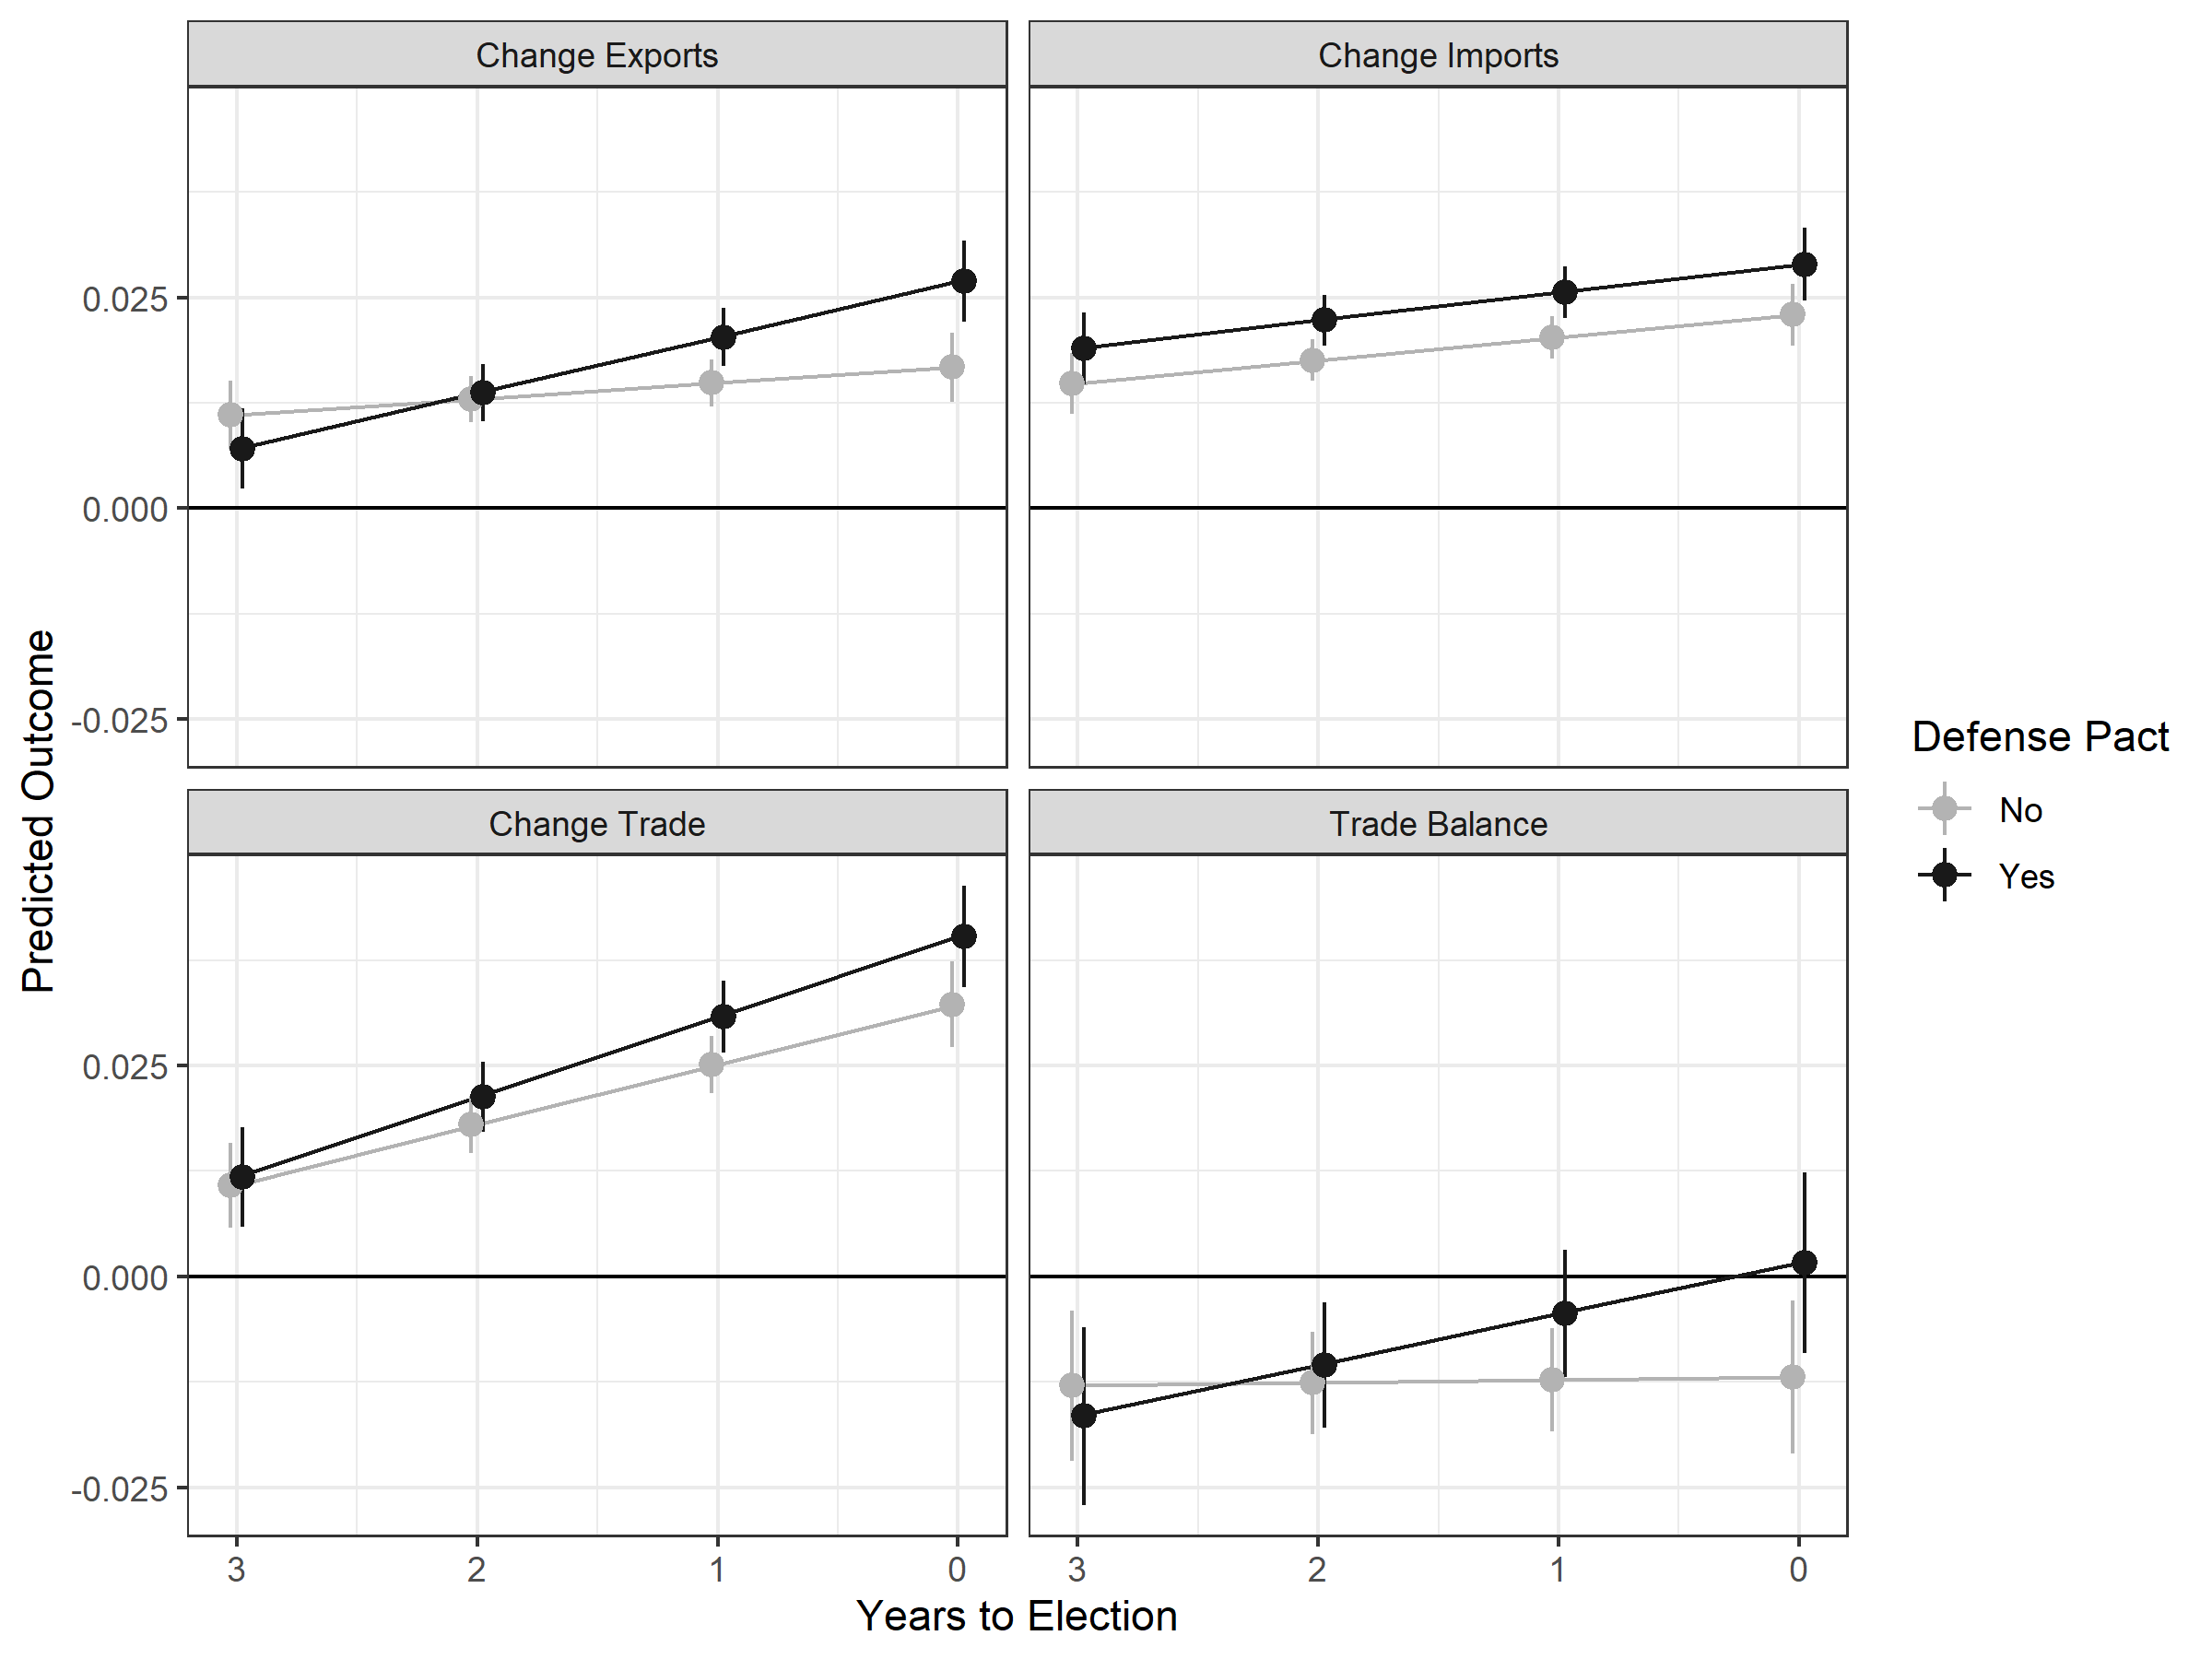
\includegraphics[width=0.95\textwidth]{../figures/us-elec-pred.png}
	\caption{Predicted changes in trade between the the United States and other states. Points mark the predictions and error bars summarize the 95\% confidence interval.}
	\label{fig:us-elec-pred}
\end{figure}


The predicted changes in exports, imports, total trade and the trade balance are consistent with inferences from the coefficient estimates. 
While U.S. exports to non-allies rise somewhat with election proximity, exports to allied states rise far more. 
Allied and non-allied export changes are comparable until the year before and year of U.S. presidential elections, and after that, allied exports increase by far more. 


% time to election
U.S. imports increase as presidential elections approach, and there is little difference in the trend between allies and other states. 
This is the result of political budget cycles boosting domestic consumption, which do not target specific goods.
Imports from allies are consistently greater than imports from non-allies, however, which is consistent with prior work on alliances and trade promotion \citep{GowaMansfield2004}. 


Differences in exports produce distinct electoral trade cycles between states with a U.S. defense treaty and those without. 
Non-allies increase imports and exports in similar ways as elections approach. 
As a result, their total trade changes increase with election proximity, but less so than allies. 


Trade balances, a common concern among some policymakers, show less evidence of electoral cycles. 
U.S. trade deficits with allies narrow somewhat around elections, but expand with non-allies, as imports rise more than exports. 
Uncertainty in these estimates makes distinguishing the estimates between and within the two groups difficult.


% improved trade balance
These results are consistent with the export cycles hypothesis. 
Exports to allies increase more near elections than exports to non-allies.
In the next analysis, I show that these differences in exports are the result of arms transfers.



\section{Arms Transfers and Presidential Elections}


I model arms transfers using data from the SIPRI Arms Transfer Database \citep{SIPRI2021}.
The outcome in this analysis is a 





\section{Discussion and Conclusion}


All three results are consistent with temporary and targeted economic concessions to support committed leaders of large alliance members around elections. 
In the appendix, I check these findings.
First, I check for non-linear relationships and adequate support in the interactions \citep{Hainmuelleretal2019}. 
%I also present inferences from Bayesian models that adjust for dyadic clustering through varying intercepts.
I also present alternative model specifications that find similar conditional relationships.


Demonstrating alliance commitment aids credible security commitments and provides contingent economic leverage. 
Alliance patrons have limited economic leverage, save when allies make temporary economic concessions to help them remain in office. 
Outside of election years, reassuring allies decreases democratic major power exports.
But when leaders offer more support, exports to allies hold up in election years and may concentrate in key constituencies.


Both perspectives on relative economic leverage in asymmetric alliances thus have some validity. 
Demonstrating security commitment often reduces exports and has no impact on allied tariffs. 
At the same time, leaders can leverage security commitments to garner allied support during elections. 


Alliances can therefore help leaders manipulate economic conditions to improve their electoral prospects. 
This finding adds an international mechanism to the political budget cycle literature.
Leaders can use international cooperation in non-economic issues to encourage other states to implement favorable economic policies. 


The argument and results reflect a general phenomenon that is more pronounced in alliances due to close economic and security relations. 
States regularly manipulate international economic ties to bolster or undermine leaders depending on their perceived stance on other issues. 
To give one example, \citet{ChyzhUrbatsch2021} show that Chinese soy tariffs reduced support for Republicans in the 2018 midterm elections. 
Allies have both motive and means to undertake similar actions. 
The security benefits of a cooperative leader motivate economic changes, and allies have many economic ties to leverage when they want to help a friendly leader. 
Future research should examine this phenomenon outside of military alliances.


These results also have implications for democratic alliance credibility and maintenance. 
A stable alliance bargain can develop if leaders anticipate the potential electoral benefits of economic ties with allies.
When leaders expect that demonstrating commitment will have electoral rewards, they will be more likely to invest in alliances. 
This also makes tolerating reduced trade leverage outside of elections worthwhile for patron state leaders.


In addition to assessing how states manipulate economic ties to support friendly leaders, future research could proceed in several directions. 
This paper presents some macro correlations, but could benefit from micro foundations. 
Are individuals more willing to make temporary economic changes that disadvantage domestic firms to support a friendly leader? 
When and how economic ties encourage alliance investments also merits further investigation.
Whether these results generalize to autocratic alliances is another worthwhile inquiry. 


In conclusion, large alliances leaders have limited and conditional economic leverage that depends on political leaders' commitment reputation and leadership competition. 
When a leader makes alliance investments, their exports to allied states increase during election years, and may concentrate in swing states. 
Otherwise, commitment reduces exports, and has no impact on structural policies like tariffs regardless of electoral pressure. 
Security preponderance thus provides less economic leverage than many observers expect, but still grants influence at critical junctures.


\newpage
\singlespace
 
\bibliography{../../MasterBibliography} 


\end{document}